\renewcommand{\typeRubriek}{loep}		

%%%%%%%%%%%%%%%%%%%%%%%%%%%%%
% informatie voor de auteur %
%%%%%%%%%%%%%%%%%%%%%%%%%%%%%
% de soorten titels opmaakmogelijkheden die de auteur kan gebruiken:
% section
% section*, betekent dat er geen nummer bij gezet wordt
% subsection
% tussentitel
% citaat
% opsomming
% nummering
% bronnen
% kader
% stellingkader (genummerd)
% stellingkadertwee (niet genummerd)
% kleurkader
% werktekst



% twee parameters voor nieuwe rubriek: titel en auteur (die mogen ook leeggelaten worden o.a. voor redactioneel)
\startNieuweRubriek{Eerstegraadsfuncties}{Johan Deprez\\ Els Vanlommel}

\startcontents[mainsections]		      % om opsomming in inhoudstafel enkel tot loep te beperken
\begin{multicols}{2}                      
\inhoudstafelLoep		                  % om inhoudstafel in te voegen



%%%%%%%%%%%%%%%%%%%%%%%%%%%%%%%%%%%%%%%%%%%%%%%%%%%%%%%%%%%%%%%%
%%%%%%%%%%%           START VAN DE TEKST               %%%%%%%%%%
%%%%%%%%%%%%%%%%%%%%%%%%%%%%%%%%%%%%%%%%%%%%%%%%%%%%%%%%%%%%%%%%

\section{In deze loep}
Eerstegraadsfuncties komen in vele gedaanten voor in het curriculum van het secundair onderwijs, verspreid over alle jaren. In de eerste graad komen functies nog niet aan bod, maar daar worden eerstegraadsfuncties wel al voorbereid met recht evenredige grootheden en eerstegraadsvergelijkingen. Het doel van deze loep is niet om een volledig overzicht te geven van alles wat gedaan wordt rond eerstegraadsfuncties. Wel willen wij een aantal losse topics opfrissen en hier en daar uitbreiden. We zochten naar relevante toepassingen, een originele insteek of kleine uitbreidingen bij de verplichte leerstof. Daarnaast wilden we ook dieper ingaan op het onderwerp regressie.

In de tweede paragraaf behandelen we kort twee relevante toepassingen van recht evenredige grootheden en eerstegraadsfuncties. Die kunnen zowel in de eerste als in de tweede graad behandeld worden. 

In paragraaf 3 komt de eerstegraadsfunctie als wiskundig model aan bod in de vorm van een trendlijn. We gaan hier dieper in op de wiskundige achtergronden en we geven enkele mooie voorbeelden. Deze leerstof wordt met de nieuwe eindtermen waarschijnlijk voor veel leerlingen verplicht in de tweede graad. 

In paragraaf 4 tonen we hoe we eigenschappen van afgeleiden, meer bepaald de kettingregel en de regel voor de afgeleide van een inverse functie, kunnen voorbereiden met eerstegraadsfuncties. Door dat te doen worden deze regels meer concreet wat leidt tot dieper inzicht. Deze leerstof komt voornamelijk in de derde graad aan bod.

Paragraaf 5 gaat vooral over veranderingsformules: hoe verandert $y$ als $x$ verandert en er een lineair verband is tussen $x$ en $y$? We doen dit voor eerstegraadsfuncties van één veranderlijke en daar leggen we ook de link naar de benadering van een kromme in de omgeving van een punt door de raaklijn in dat punt. We breiden in deze paragraaf het idee van de veranderingsformules kort uit naar eerstegraadsfuncties van twee veranderlijken. Dit is een onderwerp dat niet op het verplicht lesprogramma staat, maar het ligt niet ver over de rand. In paragraaf 5 is er zowel iets te vinden voor de tweede als voor de derde graad. 

Afsluiten doen we met een paragraaf over Q-Q plots, die veel gebruikt worden om na te gaan of een dataset normaal verdeeld is. Dit onderdeel sluit aan bij de leerstof statistiek van de derde graad.

\section{Relevante voorbeelden en toepassingen van recht evenredige grootheden en eerstegraadsfuncties}

\subsection{Thermische uitzetting van vaste stoffen en vloeistoffen}

\tussentitel{Lineaire uitzetting}
Bruggen en treinsporen zetten uit wanneer de temperatuur toeneemt en krimpen in bij afkoeling. Door thermische expansievoegen zoals die uit onderstaande figuur kunnen bruggen van lengte veranderen zonder te barsten.
\begin{center}
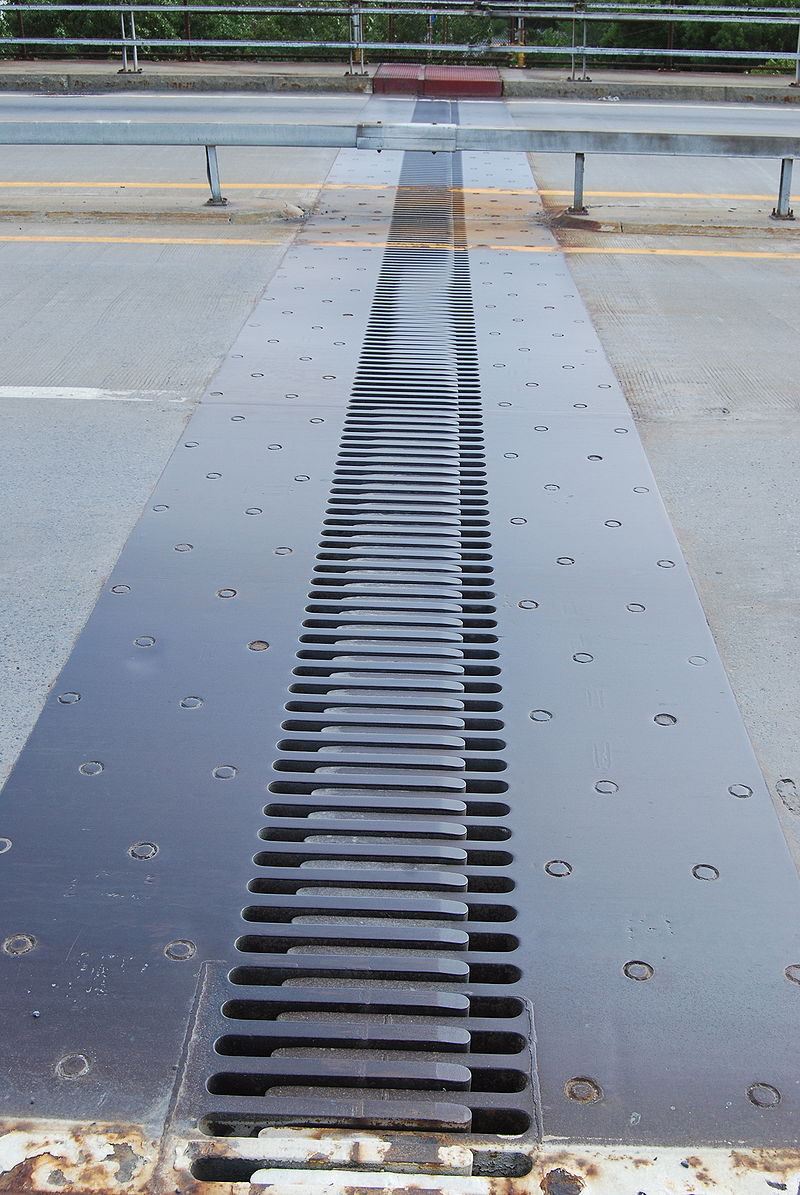
\includegraphics[width=0.8\linewidth]{figurenAuteur/thermische_expansie_voeg.jpg}
\captionof{figure}{Thermische expansievoeg op een brug in New York}
\end{center}
De verandering in lengte, $\Delta l$ (in m), is recht evenredig met de verandering in temperatuur $\Delta T$ (in graden Celsius): $$\Delta l=\alpha \cdot l_0\cdot \Delta T.$$ 

\end{multicols}

\begin{center}

\includegraphics[width=0.55\linewidth]{tekeningenKurt/Luitzetten.jpg}

\end{center}

\begin{multicols}{2}

De evenredigheidsfactoren zijn de startlengte $l_0$ (in m) en de lineaire uitzettingscoëfficiënt $\alpha$. Deze uitzettingscoëfficiënt is afhankelijk van het gebruikte materiaal en drukt uit hoeveel een meter van het materiaal uitzet bij een temperatuurstijging van 1 graad. De uitzettingscoëfficiënt van staal bijvoorbeeld, is $12\cdot 10^{-6}$ per graad Celsius. Dit wil zeggen dat 1 m staal $12\cdot  10^{-6}$ m uitzet bij een temperatuurstijging van 1 graad Celsius, of nog: $$\alpha_{\rm{staal}}=12\cdot 10^{-6}\frac{\mathrm{m}}{\mathrm{m}\cdot\; ^\circ\mathrm{C}}=12\cdot 10^{-6}\frac{1}{^\circ\mathrm{C}}.$$

De belangrijkste overspanning van de Golden Gate Bridge in San Francisco is 1275 m lang. De brug wordt blootgesteld aan temperaturen variërend van $-15^\circ$ C tot $40^\circ$ C. Neem aan dat de brug volledig van staal is gemaakt.\\

Je kunt narekenen dat het lengteverschil dan $0,84$ m is. Hoewel het niet groot is in vergelijking met de lengte van de brug, kan dit lengteverschil werkelijk waargenomen worden. In de praktijk wordt het verspreid over veel expansievoegen zodat de uitzetting bij elke voeg heel klein is.\\ 

Je kunt ook een tabel of grafiek maken voor meerdere temperatuurverschillen, bijvoorbeeld verschillen variërend van $-20^\circ$ C tot $55^\circ$ C in stappen van $5^\circ$ C.

\tussentitel{Thermische expansie in drie dimensies}
Objecten zetten uit in alle dimensies: niet alleen hun lengtes, maar ook hun volumes nemen toe met de temperatuur.

Voor de volumeverandering kennen we de volgende formule: $$\Delta V=\beta \cdot V_0 \cdot \Delta T$$ met $\Delta V$ de volumeverandering in m$^3$ en $\Delta T$ de verandering in temperatuur (in graden Celsius). De evenredigheidsfactoren zijn het startvolume $V_0$ (in m$^3$) en de kubieke uitzettingscoëfficiënt $\beta$. Die laatste is afhankelijk van het materiaal en drukt uit hoeveel een kubieke meter van het materiaal uitzet bij een temperatuurstijging van 1 graad.

Verschillen in thermische uitzetting van materialen kunnen leiden tot interessante effecten.\\ 

Een voorbeeld is het overlopen van een benzinetank van een wagen op een heel warme dag na een tankbeurt. De benzine wordt opgeslagen in grote ondergrondse tanks onder het tankstation. De temperatuur is daar koeler dan de luchttemperatuur, zeker op een warme zomerdag. Wanneer benzine getankt wordt in de stalen tank van de wagen, dan koelt deze benzine die tank. Daarna zetten zowel benzine als tank uit als ze opwarmen tot luchttemperatuur. Benzine zet echter veel meer uit dan staal. Op een heel warme zomerdag kan dit verschil zo groot worden dat een benzinetank die bijna vol gevuld is, na een tijdje kan overlopen zodat er benzine gemorst wordt.

Berekenen we bijvoorbeeld het volumeverschil voor een benzinetank van 60 liter, bij een temperatuur die toeneemt van $15^\circ$ C tot $35^\circ$ C. De tank wordt daarbij verondersteld volledig van staal te zijn. We weten ook nog dat een massieve blok staal en een holle stalen tank met hetzelfde volume even veel uitzetten. Het gemorste volume is: $$V=\Delta V_{\text{benzine}}-\Delta V_{\text{tank}}.$$ De waarden voor $\beta$ zijn $950\cdot 10^{-6}$ per graad Celsius voor de benzine en $35\cdot 10^{-6}$ per graad Celsius voor de stalen tank. Met die waarden kun je narekenen dat de gemorste hoeveelheid benzine ongeveer 1,1 liter is. Dat is toch wel aanzienlijk voor een tank van 60 liter!

\subsection{Van Celsius naar Fahrenheit}
Daniel Gabriel Fahrenheit bedacht in 1724 een temperatuurschaal die nu nog steeds vooral in de Verenigde Staten wordt gebruikt. Enkele jaren later, in 1742, definieerde Anders Celsius de temperatuurverdeling in graden Celsius.

De omzettingsformule om van graden Celsius naar Fahrenheit te gaan, is $$T_F=32+\frac{9}{5}\cdot T_C.$$
Hiermee komt de eerstegraadsfunctie $f(x)=32+\frac{9}{5}\cdot x$ overeen. Wat is de betekenis van de $y$-coördinaat van het snijpunt met de verticale as? En hoe moeten we de andere term interpreteren?

\end{multicols}

\begin{center}
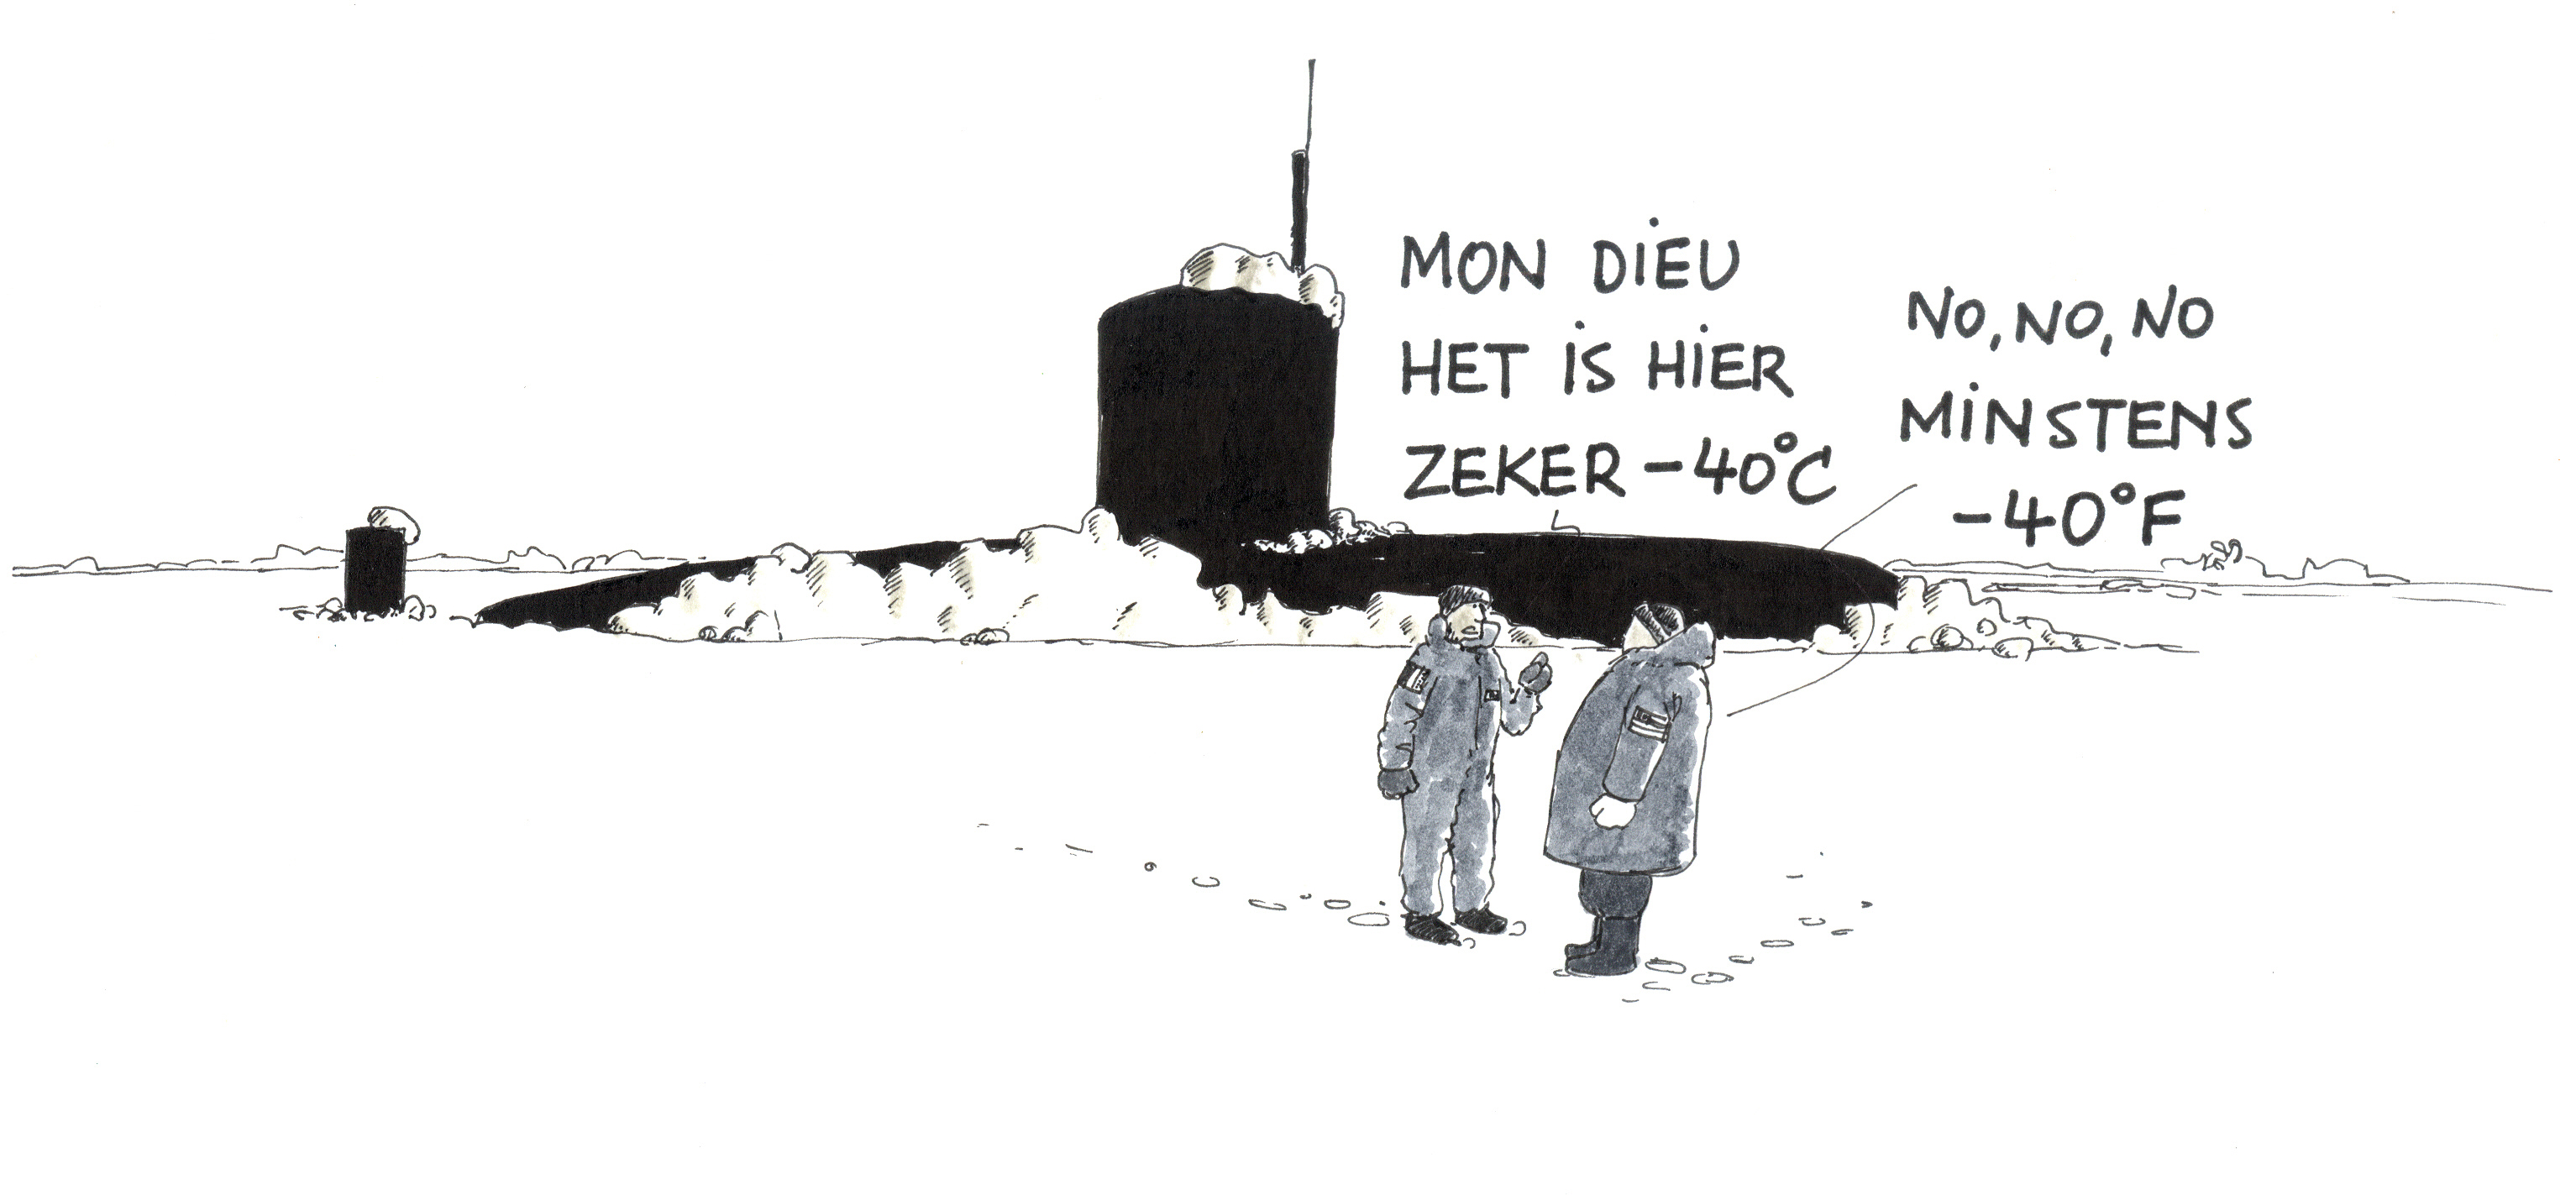
\includegraphics[width=\linewidth]{tekeningenKurt/Ltemperaturen.jpg}

\end{center}

\begin{multicols}{2}

De $y$-coördinaat van het snijpunt met de verticale as (dit wordt soms ook wel het intercept genoemd), 32, komt overeen met de smelttemperatuur van ijs. De andere term is evenredig met het aantal graden Celsius. De richtingscoëfficiënt $\frac{9}{5}$ is de evenredigheidsfactor. Dit betekent dat een toename van de temperatuur met één graad Celsius overeenkomt met een toename van $\frac{9}{5}$ graden Fahrenheit.

Kan een temperatuur gelijk zijn bij beide schalen? Zo ja, bij welke temperatuur is dat?\\

Om het antwoord te vinden op deze vraag, moeten we de eerstegraadsvergelijking $T_F=T_C$ oplossen. We vinden dat bij -40 graden de temperatuur gelijk is bij beide schalen.

\subsection{Kosten, ontvangsten en winst}

Niet alleen in de natuurwetenschappen, maar ook in de economie worden eerstegraadsfuncties vaak gebruikt. In deze paragraaf bespreken we enkele van de vele voorbeelden. Om een product te kunnen produceren en aan de man te brengen, moet een firma kosten maken. Een deel hiervan zijn vaste kosten: ze hangen niet af van de geproduceerde hoeveelheid. Denk bijvoorbeeld aan de huur van de fabriekshal: die moet de firma in elk geval betalen, ook als er niets geproduceerd zou worden. Daarnaast zijn er variabele kosten, die wel afhangen van de hoeveelheid die geproduceerd en verkocht wordt. Dat kunnen bijvoorbeeld kosten zijn voor de grondstoffen, loonkosten, … Vaak ligt het voor de hand om aan te nemen dat de variabele kosten evenredig zijn met de hoeveelheid. De kostenfunctie heeft dan de volgende structuur:

totale kosten

$=$ vaste kosten $+$ vast bedrag $\cdot$ aantal eenheden.

Dat vaste bedrag is de supplementaire kost per bijkomende eenheid en het wordt de marginale kostprijs genoemd. De kostenfunctie is dan een eerstegraadsfunctie. In formulevorm krijgen we dan dat $K=b+a\cdot q$, met $K$ de totale kosten, $q$ het aantal eenheden dat geproduceerd en verkocht wordt en $a$ en $b$ positieve getallen. De coëffi\-ciënten $a$ en $b$ krijgen in deze context een mooie interpretatie (marginale kost en vaste kost), die in een verwante vorm terugkomt in veel andere contexten (vast recht en prijs per kilowattuur, startwaarde en wat erbij komt of eraf gaat per uur, …). Bemerk dat het hier natuurlijker aanvoelt om de constante term eerst te schrijven.

Ook de ontvangsten bij de verkoop kunnen we weergeven met een eerstegraadsfunctie: die zijn immers evenredig met het aantal verkochte eenheden. Zo krijgen we dat $O=c\cdot q$, waarbij $O$ de ontvangsten voorstelt en $c$ de verkoopprijs per eenheid (waarbij we hopen dat $c>a$). De gemaakte winst vinden we door beide functies te combineren: $W=O-K=-b+(c-a) \cdot q$, met $W$ de winst. Ook deze winstfunctie is een eerstegraadsfunctie. We zien een startwaarde, die in dit geval negatief is (de vaste kosten zorgen dat we verlies maken als we niets produceren en verkopen), en een vast bedrag dat erbij komt voor elke eenheid die we verkopen (de marginale winst $c-a$).

De vraag die hier voor de hand ligt, is vanaf welke hoeveelheid we effectief winst maken. In een derdejaarsklas werk je met een concreet voorbeeld. Wij houden het nu contextloos, maar nemen wel concrete waarden voor de parameters: $b=960$, $a=5$ en $c=8$. We lossen de vraag op twee verschillende manieren grafisch op. Eerst maken we gebruik van de winstfunctie $W=-960+3q$: we onderzoeken voor welke waarden de grafiek boven de horizontale as ligt (zie de grafiek in figuur \ref{geld1}). We vinden dat de firma break-even draait (d.w.z. zonder winst of verlies) als $q=320$ en effectief winst maakt voor grotere waarden van $q$. Bij de tweede manier onderzoeken we vanaf welke waarde van $q$ de grafiek van de opbrengstenfunctie hoger ligt dan die van de kostenfunctie (zie de grafiek in figuur \ref{geld2}). We lossen dus de ongelijkheid $9q\geq 960+5q$ op, zonder eerst alles naar het linkerlid te brengen. Uiteraard vinden we dezelfde uitkomst.

\begin{center}
\includegraphics[width=0.85\linewidth]{figurenAuteur/geld1.png}
\captionof{figure}{Een winstgrafiek door het break-even-punt}{\label{geld1}}
\end{center}

\begin{center}
\includegraphics[width=0.85\linewidth]{figurenAuteur/geld2.png}
\captionof{figure}{Een kostengrafiek en een ontvangstgrafiek door het break-even-punt}{\label{geld2}}
\end{center}

We staan tot slot nog even stil bij deze twee manieren van werken, die in principe bij elke vergelijking of ongelijkheid mogelijk zijn. In dit geval liggen ze beide voor de hand. In andere situaties, bijvoorbeeld het zoeken van het evenwicht tussen vraag en aanbod, kun je beter blijven werken met de aparte functies, zonder de vergelijking eerst op 0 te herleiden, omdat het verschil tussen vraag en aanbod geen directe betekenis heeft.


\section{Eerstegraadsfuncties als wiskundig model: rechte als trendlijn}
Een van de nieuwe eindtermen voor studierichtingen uit de tweede graad met doorstroomfinaliteit (d.w.z. de huidige aso-studierichtingen en een aantal tso/kso-studierichtingen) schrijft voor dat leerlingen het verband tussen twee numerieke grootheden in een dataset moeten kunnen onderzoeken: ze moeten de data in een spreidings\-diagram kunnen voorstellen en ze moeten een gepaste trendlijn kunnen bepalen met behulp van ICT (nog onder voorbehoud, want de nieuwe eindtermen zijn nog niet finaal goedgekeurd). Met de trendlijn wordt de regressielijn bedoeld, die bepaald wordt met de kleinste-kwadraten-methode. Deze eindterm is onder andere van belang in functie van de wetenschapsvakken, waarin leerlingen verbanden moeten kunnen bepalen op basis van experimentele data, maar ook in economie en humane wetenschappen worden trendlijnen frequent gebruikt. Zoals de eindterm geformuleerd is, hoort hij thuis onder de beschrijvende statistiek, maar er is een evidente link naar functies: zo’n trendlijn is de grafiek van een functie. En in deze loep bekijken we natuurlijk hoe we eerstegraadsfuncties in verband kunnen brengen met deze eindterm.

De trendlijn wordt met behulp van ICT bepaald. De meest voor de hand liggende hulpmiddelen zijn dan een grafische rekenmachine en een rekenblad (Excel, LibreOffice Calc, GNumeric, …). De rekentechnische kant blijft daardoor erg beperkt en komt in deze paragraaf niet expliciet aan bod. Dat biedt de gelegenheid om tijdens de lessen vooral in te zoomen op een aantal meer conceptuele aspecten en dat is wat we in dit deel van de loep uitwerken.

\subsection{Een functie als wiskundig model}
Tegenwoordig worden leerlingen er al vroeg vertrouwd mee gemaakt dat functies gebruikt worden om fenomenen uit de realiteit te beschrijven. In die toepassingen is de functie in kwestie meestal gegeven, bijvoorbeeld in formulevorm of via een andere representatie die leerlingen dan moeten gebruiken om het voorschrift op te stellen. De eindterm over de trendlijn biedt de gelegenheid om met de leerlingen dieper in te gaan op het zelf zoeken van een geschikte functie: welk type van functie is geschikt en hoe vind je binnen dit type een gepaste functie?

Leerlingen moeten dus zelf een wiskundig model opstellen. Daarbij worden ze er nadrukkelijk mee geconfronteerd dat zo’n wiskundig model altijd een vereenvoudiging is: het is een idealisering die de realiteit slechts bij benadering beschrijft. In het begin kan dat verwarrend zijn voor de leerlingen. Deze manier van werken staat immers haaks op wat we gewoon zijn binnen de zuivere wiskunde. Daar leggen we immers juist de nadruk op exactheid. Daarom is het goed om in de les toch wat tijd uit te trekken om leerlingen vertrouwd te laten worden met deze nieuwe manier van werken. In deze loep werken we dat niet uit omdat we dat al eerder gedaan hebben. We hebben namelijk al eens een loep specifiek gewijd aan modelleren (Deprez, Op de Beeck en Van den Broeck, 2011). Daarin hebben we in detail uitgewerkt hoe je tijdens de les het modelleren kunt introduceren via eerstegraadsfuncties.

In die eerdere loep hebben we de trendlijn op een heel informele manier bepaald: we bepaalden een rechte die de punten in het spreidingsdiagram op het zicht goed weergaf. Ook nu we in het kader van de nieuwe eindterm de trendlijn met ICT zullen bepalen, vinden we het zinvol om in het begin even met deze heel intuïtieve manier te werken. Die laat immers een van de aspecten van het modelleren goed aanvoelen: we mogen het model niet verabsoluteren; elk model is maar één van de vele mogelijke modellen.

\subsection{Drie voorbeelden}
Goede voorbeelden zijn van groot belang bij het leren van statistiek. We willen data in een zinvolle context waarbinnen het ook zinvol is om een trendlijn te zoeken. Anderzijds zochten we voorbeelden in functie van wat we vanuit wiskundig standpunt wilden uitwerken. Alle voorbeelden in deze paragraaf zijn gebaseerd op data die we vonden op de website `Data and Story Library’, die zich toelegt op het verzamelen van goede voorbeelden voor statistiekonderwijs. Je vindt het adres van deze website in de bibliografie van deze loep. Je vindt nog meer inspiratie in een loep die we lang geleden maakten over regressie (Deprez, Roels en Tytgat, 2005).

Zoals eerder gezegd, gaan we in deze paragraaf niet in op de concrete handelingen die je moet uitvoeren om een spreidingsdiagram te maken en een trendlijn te tekenen, maar richten onze aandacht op het interpreteren van de coëfficiënten en de vraag of de trendlijn zinvol is. 

\tussentitel{Voorbeeld 1: rokers}
De dataset uit de tabel hieronder toont de evolutie van het percentage rokers bij 18-24-jarige mannen en vrouwen in de VS tussen 1999 en 2014. Je vindt de dataset ook in digitale vorm op onze website.
\begin{center}
\includegraphics[width=0.5\linewidth]{figurenAuteur/vbregressie1.png}
\captionof{figure}{Evolutie van het percentage rokers bij 18-24-jarige mannen en vrouwen in de VS}
\end{center}
We laten de leerlingen eerst een spreidingsdiagram maken met daarin beide tijdreeksen. We laten hen ook de bijbehorende trendlijnen bepalen, evenals de waarde van $R^2$. Het resultaat (met Excel) vind je in figuur \ref{reg2}.
\begin{center}
\includegraphics[width=1\linewidth]{figurenAuteur/vbregressie2.png}
\captionof{figure}{Twee dalende trendlijnen}{\label{reg2}}
\end{center}
Merk op dat we hier werken met de determinatiecoëfficiënt $R^2$ i.p.v. met de correlatiecoëfficiënt. In het geval van een lineaire trendlijn is $R^2$ gewoon het kwadraat van de correlatiecoëfficiënt. De interpretatie loopt dus gelijk met die van de correlatiecoëfficiënt: hoe dichter $R^2$ bij $1$ ligt, hoe beter de rechte aansluit bij de datapunten. Het voordeel van de determinatiecoëfficiënt is dat hij wel nog gedefinieerd kan worden bij een niet-lineaire trendlijn, maar de correlatiecoëfficiënt niet.

Het maken van het spreidingsdiagram en het opstellen van de trendlijn is niet het einde van de oefening. Integendeel, het belangrijkste werk moet nog komen: de interpretatie van de resultaten. Daarbij passeren allerlei elementen de revue, bijvoorbeeld: de coëfficiënten in de vergelijking van de trendlijn, de waarde van $R^2$ en het maken van voorspellingen met de trendlijn.

De richtingscoëfficiënt in de trendlijn bij de vrouwen betekent dat het percentage rokers bij hen elk jaar met (afgerond) $0,76$ procentpunt afneemt. We gebruiken hier bewust het woord `procentpunt’ i.p.v. `procent’ om verwarring te vermijden: het gaat immers over een absolute afname (je trekt $0,76$ af van het percentage), niet over een relatieve afname (waarbij je het percentage zou vermenigvuldigen met $1-\frac{0,76}{100}$). De richtingscoëfficiënt in de trendlijn bij de mannen toont dat het percentage rokers bij hen iets trager afneemt dan bij de vrouwen. Omdat het verschil klein is, moet je al goed kijken om dat op de grafiek te kunnen aflezen. 

Met de vergelijkingen van de trendlijnen kun je nu ook voorspellingen maken (of terugrekenen in de tijd). Sommige van die voorspellingen zijn zinvol (bijvoorbeeld: wanneer je mag verwachten dat het aantal rokers bij mannen en vrouwen onder de $10\%$ gezakt zal zijn), maar als je te ver in de toekomst (of in het verleden) kijkt, moet je je afvragen of de daling uit de dataset wel aangehouden zal kunnen worden. Het is dus wel duidelijk dat de constante term in de vergelijking van de trendlijnen in dit geval geen concrete betekenis heeft. Het zou een argument kunnen zijn om de tijd anders weer te geven, bijvoorbeeld met een tijdschaal die start in 1999.

We merken dat de waarde van $R^2$ bij de vrouwen een stuk groter is dan die bij de mannen. Dat is in overeenstemming met wat we in het spreidingsdiagram zien: de datapunten bij de vrouwen sluiten veel beter aan bij de rechte dan de datapunten bij de mannen.

Je moet zeker nog meer rechttoe-rechtaan-voorbeelden zoals dit behandelen, waarbij de trendlijn een goede beschrijving geeft van de datapunten en waarbij je de coëfficiënten van de trendlijn laat interpreteren en een voorspelling laat maken. Mits wat zoeken vind je hiervoor goede data en contexten. De volgende twee voorbeelden liggen wat minder voor de hand: eerst laten we zien dat een rechte trendlijn niet altijd een goede beschrijving van de datapunten geeft en vervolgens geven we een voorbeeld waarin een rechte trendlijn tegen de verwachtingen in toch zinvol is.

\tussentitel{Voorbeeld 2: prijzen van externe harde schijven}
De dataset uit de volgende tabel toont de grootte en de prijs van een aantal externe harde schijven, zoals genoteerd op Amazon.com in 2016.
\begin{center}
\includegraphics[width=0.65\linewidth]{figurenAuteur/vbregressie3.png}
\captionof{figure}{Grootte en prijs van externe harde schijven bij Amazon.com in 2016}
\end{center}
We laten de leerlingen eerst het spreidingsdiagram maken en de trendlijn bepalen van de externe harde schijven tot en met 4 TB (zie figuur \ref{reg4}). We krijgen een goed bruikbare trendlijn, die laat zien dat elke extra TB aanleiding geeft tot een bijkomende kostprijs van (afgerond) $23$ dollar.

\begin{center}
\includegraphics[width=\linewidth]{figurenAuteur/vbregressie4.png}
\captionof{figure}{Een stijgende trendlijn voor kleine harde schijven}{\label{reg4}}
\end{center}
Ook voor de harde schijven van 4 t.e.m. 12 TB krijgen we een goed bruikbare trendlijn, maar in deze categorie van grootte betaal je (afgerond) 114 dollar per bijkomende TB (zie figuur \ref{reg5}).

Wil je de grootste harde schijf die te koop is, dan moet je voor de extra terabytes nog meer investeren: met de gegevens in de tabel kun je nagaan dat de sprong van 12 naar 32 TB een bijkomende kost van (afgerond) 169 dollar per TB met zich meebrengt.

\begin{center}
\includegraphics[width=\linewidth]{figurenAuteur/vbregressie5.png}
\captionof{figure}{Een stijgende trendlijn voor middelgrote harde schijven}{\label{reg5}}
\end{center}

Op basis van het voorgaande valt te verwachten dat de we geen trendlijn zullen vinden die de volledige dataset goed weergeeft. Figuur \ref{reg6} bevestigt dit, ook al heeft $R^2$ een waarde die dicht bij 1 ligt.
\begin{center}
\includegraphics[width=\linewidth]{figurenAuteur/vbregressie6.png}
\captionof{figure}{Een trendlijn voor grote en kleine harde schijven}{\label{reg6}}
\end{center}

\tussentitel{Voorbeeld 3: regenval in Los Angeles}
Figuur \ref{reg7} toont de evolutie van de jaarlijkse hoeveelheid neerslag (in mm) in Los Angeles (we geven de data zelf hier niet, maar je vindt ze wel op onze website).

Het is wel duidelijk dat er heel wat variatie in de neerslaghoeveelheden zit en dat de datapunten zeker niet allemaal dicht bij eenzelfde rechte liggen. De waarde voor $R^2$ zal zeker niet dicht bij $1$ liggen. Toch levert de trendlijn hier interessante informatie, zoals figuur \ref{reg8} duidelijk maakt: ze laat ons vermoeden dat er doorheen alle variatie misschien toch wel een dalende trend aanwezig is.
\begin{center}
\includegraphics[width=\linewidth]{figurenAuteur/vbregressie7.png}
\captionof{figure}{\label{reg7}}
\end{center}

\begin{center}
\includegraphics[width=\linewidth]{figurenAuteur/vbregressie8.png}
\captionof{figure}{Dalende trend in een diffuse puntenwolk}{\label{reg8}}
\end{center}


\subsection{Hoe wordt de trendlijn bepaald?}
De trendlijn uit de eindterm is de regressielijn die bepaald wordt via de kleinste-kwadraten-methode. In het kader van de eindterm hoef je op deze methode niet in te gaan en blijft het bepalen van de regressielijn dus een black box. Daar is niets op tegen. Ook het berekenen van een vierkantswortel met de rekenmachine, om maar iets te noemen, blijft voor de leerlingen een black box, zonder dat we ons daar zorgen over maken. En we hopen je er ondertussen ook van overtuigd te hebben dat er best wel interessante, wiskundige zaken te doen zijn rond de trendlijn zonder daarom te weten hoe die precies bepaald wordt. Een volledige afleiding van de kleinste-kwadraten-methode, met alles erop en eraan, overstijgt trouwens de leerstof uit het secundair onderwijs, bijvoorbeeld omdat er gebruik gemaakt wordt van functies van meerdere veranderlijken. 

Hoewel het dus niet per se hoeft, en het niet in zijn volledigheid kan, zijn er toch interessante mogelijkheden om een tip van de sluier op te lichten in de tweede graad van het secundair onderwijs. Dat is wat we in deze paragraaf willen tonen. We hebben hiervoor een GeoGebra-applet uitgewerkt.


\end{multicols}
\begin{center}
\includegraphics[width=1\linewidth]{figurenAuteur/rekenblad1.png}
\captionof{figure}{De gegevens in een puntenwolk samen met het zwaartepunt}{\label{reken1}}
\end{center}
\begin{multicols}{2}

\tussentitel{De rechte}
Als je het vakje `rechte tonen’ aanvinkt, krijg je een rechte te zien die door het zwaartepunt gaat (zie figuur \ref{reken2}). Er is ook een schuifknop waarmee je de waarde van $a$ kunt instellen. De eerstegraadsfunctie die overeenkomt met de getekende rechte heeft dus als vergelijking $f(x)=y_M+a\left(x-x_M\right)$, waarbij $\left(x_M,\ y_M\right)$ het zwaartepunt is en $a$ de waarde die met de schuifbalk vastgelegd is. Het is duidelijk dat de waarde van $b$ bepaald is eens de waarde van $a$ gekozen is.

\tussentitel{De GeoGebra-applet: de data en een vereenvoudiging}
De data waar we in de GeoGebra-applet mee werken, vind je in kolommen B en C van het (rekenblad)venster aan de rechterkant (zie figuur \ref{reken1}). Het spreidingsdiagram vind je in het middelste (teken)venster. In het linkse (teken)venster zie je voorlopig niets.
\end{multicols}
\begin{center}
\includegraphics[width=\linewidth]{figurenAuteur/rekenblad2.png}
\captionof{figure}{En samen met een kandidaat voor de best passende kromme}{\label{reken2}}
\end{center}
\begin{multicols}{2}


Een eerstegraadsfunctie wordt bepaald door twee parameters: de coëfficiënten $a$ en $b$ in het voorschrift $f\left(x\right)=ax+b$. Je kunt die twee parameters echter eenvoudig reduceren tot één parameter als je bereid bent te steunen op een eenvoudige eigenschap van de trendlijn die we hier niet bewijzen: de trendlijn gaat door het `zwaartepunt’ van de puntenwolk (zie het rode kruis in figuur \ref{reken1}; de kleur zie je in de gedrukte versie van dit artikel niet, maar wel in de digitale versie van het artikel op onze website en in de applet zelf). De $x$-coördinaat van dat zwaartepunt is het gemiddelde $x_M$ van de $x$-waarden uit de dataset en zijn $y$-coördinaat is het gemiddelde $y_M$ van de $y$-waarden van de dataset. In de applet maken we gebruik van deze vereenvoudiging. Op het einde van deze paragraaf komen we nog even terug op deze vereenvoudiging.

Met wat je nu in de applet ziet, kun je al proberen om een geschikte waarde voor $a$ te vinden. Er is natuurlijk geen rechte die exact door alle datapunten gaat. Je probeert dus een rechte te vinden die zo goed mogelijk bij de punten aansluit, waarbij de beoordeling voorlopig puur visueel gebeurt.

\tussentitel{De kleinste-kwadraten-methode gevisualiseerd}
De kleinste-kwadraten-methode geeft een getalsmatig beoordelingscriterium voor het bepalen van de waarde van $a$:
\begin{itemize}
    \item er wordt (op een welbepaalde manier, die we hieronder zullen uitleggen) een getal berekend dat meet hoe sterk de rechte van de punten afwijkt;
    \item dat getal hangt af van de waarde van $a$;
    \item voor $a$ kiezen we dan de waarde waarvoor dit getal zo klein mogelijk is.
\end{itemize}
We werken dit hieronder stap voor stap uit aan de hand van de applet.

We starten met het aanvinken van het vakje `lijnstukken tonen’, waardoor er in de applet lijnstukjes getoond worden die de datapunten verticaal verbinden met de rechte (zie figuur \ref{reken3}). Hoe langer deze lijnstukjes zijn, hoe meer de rechte afwijkt van de datapunten. We bekijken daarom hoe je hun lengte kunt bepalen. De lengte van zo’n verticaal lijnstukje is de absolute waarde van het verschil tussen de $y$-coördinaten van zijn twee randpunten. Het ene randpunt is het datapunt, waarvan de $y$-coördinaat gegeven is (zie kolom C in het rekenblad). De $y$-coördinaat van het andere randpunt is niet onmiddellijk gegeven, maar zijn $x$-coördinaat is gelijk aan die van het datapunt. Omdat dit andere randpunt bovendien op de rechte ligt, is zijn $y$-coördinaat dan gelijk aan de functiewaarde van deze $x$-coördinaat volgens de bijbehorende eerstegraadsfunctie (dus gelijk aan $f(x_i)=y_M+a\left(x_i-x_M\right)$, waarin $x_i$ de $x$-waarde van de het $i$-de datapunt is en $a$ de waarde die met de schuifbalk vastgelegd is). Je vindt deze $y$-waarden ook terug in het rekenblad: zie kolom D. De lengte van de groene lijnstukjes vind je in kolom E. We kunnen de betekenis van de lengte van zo’n lijnstukje nu preciezer als volgt omschrijven: ze geeft aan hoe sterk de $y$-waarde volgens de rechte afwijkt van de $y$-waarde van het datapunt.

We vinken nu het vakje `vierkanten tonen’ aan. Aan elk lijnstukje is nu een vierkant gehecht en onderaan in de figuur wordt de totale oppervlakte van al deze figuren getoond. Ook in het rekenblad wordt de oppervlakte berekend: in kolom F vind je de kwadraten van de getallen uit kolom E. Deze getallen geven dus de oppervlaktes van de vierkanten. Onderaan vind je de som van al die getallen, d.w.z. de totale oppervlakte van alle vierkanten.

Welke betekenis kunnen we aan deze totale oppervlakte hechten? We kennen reeds de betekenis van de lengte van een groen lijnstukje: hoe langer het lijnstuk, hoe groter de afwijking tussen de $y$-waarde volgens de rechte en de y-waarde van het datapunt. De overgang naar het vierkant betekent dat we deze lengte kwadrateren. In het totaal wegen grote afwijkingen daardoor sterker door dan kleine afwijkingen. We besluiten dat de totale oppervlakte van alle vierkanten een maat is voor de `totale afwijking’ tussen de rechte en de datapunten. Daarom is het deze totale oppervlakte van de vierkanten die we zo klein mogelijk proberen te maken.

Met wat je nu in de applet ziet, kun je nu opnieuw proberen om een geschikte waarde voor $a$ te vinden. Probeer hierbij nu dus de totale oppervlakte zo klein mogelijk te maken.
\end{multicols}
\begin{center}
\includegraphics[width=\linewidth]{figurenAuteur/rekenblad3.png}
\captionof{figure}{Visualisering van de som van de kwadratische afwijkingen}{\label{reken3}}
\end{center}
\begin{multicols}{2}

\tussentitel{Een parabool}
Vink tot slot het vakje `grafiek tonen’ aan. In het linkse venster zie je nu een parabool (zie figuur \ref{reken4}). Deze parabool toont hoe de totale oppervlakte van de vierkanten (uitgezet op de verticale as) samenhangt met de waarde van $a$ (uitgezet op de horizontale as). Dit geeft meer inzicht bij het zoeken naar de optimale waarde van $a$. Het komt er dus blijkbaar op aan om het eerste coördinaatgetal van de top van de parabool te bepalen!
\end{multicols}
\begin{center}
\includegraphics[width=\linewidth]{figurenAuteur/rekenblad4.png}
\captionof{figure}{\label{reken4}}
\end{center}
\begin{multicols}{2}
We hebben hiermee natuurlijk nog niet verklaard waarom de grafiek een parabool is. Voor een kleine en concrete dataset kun je dat misschien nog met de leerlingen doen, maar de algemene redenering is in de tweede graad wellicht een brug te ver. Voor de volledigheid geven we ze hier wel, voor een algemene dataset, maar dus wel vertrekkend van de eigenschap dat de regressierechte door het zwaartepunt van de dataset gaat. Als je alles bijeenbrengt wat we hierboven besproken hebben, vind je (geformuleerd voor een dataset met $n$ punten):
\begin{align*}
\text{opp}	&=\left(y_1-f\left(x_1\right)\right)^2+\cdots+\left(y_n-f\left(x_n\right)\right)^2\\               &=\left(y_1-\left(y_M+a\left(x_1-x_M\right)\right)\right)^2+\cdots\\                          &\qquad  +\left(y_n-\left(y_M+a\left(x_n-x_M\right)\right)\right)^2\\
           &=\left(\left(y_1-y_M\right)-a\left(x_1-x_M\right)\right)^2+\ldots\\
           &\qquad  +\left(\left(y_n-y_M\right)-a\left(x_n-x_M\right)\right)^2\\
           &=A\cdot a^2+B\cdot a+C
\end{align*}
met
\begin{align*}
    A&=\left(x_1-x_M\right)^2+\ldots+\left(x_n-x_M\right)^2\\
    &=\sum_{i=1}^{n}\left(x_i-x_M\right)^2,\\
    B&=-2\cdot\Big(\left(x_1-x_M\right)\left(y_1-y_M\right)+\cdots\\
    &\qquad +\left(x_n-x_M\right)\left(y_n-y_M\right) \Big)\\
    &=-2\sum_{i=1}^{n}{(x_1-x_M)(y_1-y_M)} \text{\ \ \  en}\\
    C&=\left(y_1-y_M\right)^2+\cdots+\left(y_n-y_M\right)^2\\
    &=\sum_{i=1}^{n}\left(y_i-y_M\right)^2.
\end{align*}

Nu we zo ver geraakt zijn, kunnen we het natuurlijk niet laten om ook de formule voor de optimale waarde van $a$ af te leiden:
\begin{align*}
    a&=-\frac{B}{2A}\\
    &=\frac{\sum_{i=1}^{n}\left(x_1-x_M\right)\left(y_1-y_M\right)}{\sum_{i=1}^{n}\left(x_i-x_M\right)^2}\\
    &=\frac{\text{cov}(x,y)}{\text{var}(x,y)}.
\end{align*}
De parameter $b$ kan (zoals voorheen) eenvoudig bepaald worden via $b=y_M-ax_M$.

\tussentitel{Terug naar onze vereenvoudiging}
De gedachtegang die we hierboven ontwikkeld hebben, steunt op de eigenschap dat de regressierechte door het zwaartepunt van de datapunten gaat. Op de GeoGebra-website vind je tal van applets die de kleinste-kwadraten-methode visualiseren met vierkanten zonder gebruik te maken van deze vereenvoudiging. Je vindt dan twee schuifbalken, een voor $a$ en een voor $b$. De eerste stappen uit de opbouw die we hierboven geschetst hebben, kun je met deze applets ook doen. De laatste stap, de overgang naar de parabool, kun je dan echter niet meer zetten. De totale oppervlakte van de vierkanten hangt nu immers af van twee variabelen: zowel $a$ als $b$. De grafiek is nu een oppervlak in de driedimensionale ruimte (meer bepaald: een elliptische paraboloïde, als grafiek van een tweedegraadsfunctie van twee variabelen). Het bepalen van de optimale waarde van $a$ en $b$ via de grafiek wordt hierdoor in de praktijk ondoenbaar. Wat in deze algemene situatie wel kan, is het bepalen van de optimale waarde via een tabel. Op onze website vind je een rekenblad waarin dit uitgewerkt is: in een 2-dimensionale tabel wordt de totale oppervlakte van de vierkanten getoond als functie van $a$ en $b$ en worden de optimale waarden aangeduid.



\section{Eigenschappen van afgeleiden voorbereiden}
De afgeleide van een functie in een punt is de richtingscoëfficiënt van de raaklijn in dat punt en die raaklijn is een lineaire benadering van de functie in dat punt. Het is daarom voor de hand liggend en zinvol om sommige eigenschappen van afgeleiden in te leiden met eerstegraadsfuncties. Leerlingen krijgen op die manier meer intuïtie voor die eigenschappen. We illustreren dit met twee voorbeelden.


\subsection{Samenstellen van eerstegraadsfuncties}

In de volgende korte lesactiviteit onderzoeken de leerlingen de samengestelde van twee eerstegraadsfuncties. Dit is een voorafspiegeling van de kettingregel voor het bepalen van de afgeleide van de samengestelde van twee functies. 

Als $f$ afleidbaar is in $x$ en $g$ afleidbaar in $u=f(x)$, met $y=g(u)=h(x)$, dan is $h=g \circ f$ afleidbaar in $x$ en dan geldt: $$\frac{\mathrm{d}y}{\mathrm{d}x}=\frac{\mathrm{d}y}{\mathrm{d}u}\cdot \frac{\mathrm{d}u}{\mathrm{d}x}$$ of nog $$h'(x)=g'(u)\cdot f'(x).$$

\newpage
Voor eerstegraadsfuncties $f$ en $g$ is deze regel heel eenvoudig. Daarom is dat een mooi opstapje naar het echte werk met krommen die hellingen hebben die niet constant zijn. Voor deze lesactiviteit moeten de leerlingen nog geen afgeleiden kennen.

\begin{center}
\includegraphics[width=\linewidth]{figurenAuteur/kettingregel_fig}
\captionof{figure}{Een pijlenvoorstelling van de samengestelde van twee functies}
\end{center}



\end{multicols}

\beginwerktekst{Samenstellen van eerstegraadsfuncties}

\begin{werktekstoef}
\item{Bereken de samengestelde $h=f\circ g$ van de eerstegraadsfuncties $f:x\mapsto 3x+7$ en $g:x\mapsto 2x+1$.\\ Is die samengestelde opnieuw een eerstegraadsfunctie?}

\emph{Ja: 
\begin{align*}
    h(x)&= \left( f\circ g\right)(x)\\
    &=f\left(g(x)\right)\\
    &=f\left( 2x+1\right)\\
    &=3\left(2x+1\right)+7\\
    &=6x+10
\end{align*}}

\item{Wat stel je vast voor de richtingscoëfficiënt van de grafiek van de samengestelde functie $h$?}

\emph{De helling van de rechte die de grafiek is van $h=f\circ g$ is gelijk aan het product van de helling van de rechte die hoort bij $f$ met die van de rechte die de grafiek is van $g$. }


\item{Bepaal het voorschrift van $g\circ f$. Wat stel je vast? Is $f\circ g = g\circ f$?}

\emph{Nee:
\begin{align*}
    \left( g\circ f\right)(x)&=g\left(f(x)\right)\\
    &=g\left( 3x+7\right)\\
    &=2\left(3x+7\right)+1\\
    &=6x+15
\end{align*} De richtingscoëfficiënten blijven gelijk, maar het snijpunt met de verticale as is veranderd.}

%\emph{het antwoord}
\item{Is het altijd zo dat de samengestelde van twee eerstegraadsfuncties een eerstegraadsfunctie is? Bewijs je antwoord.}

\emph{De samengestelde functie is opnieuw een eerstegraadsfunctie omdat die samenstelling neerkomt op het vermenigvuldigen van de binnenste functie met een constante en dan vermeerderen met een constante. Het resultaat blijft dus van de eerste graad. \\Dit kun je ook algebraïsch bewijzen. \\Stel $f(x)=ax+b$ en $g(x)=cx+d$ met $a\neq 0$ en $c\neq 0$. Dan:
\begin{align*}
    h(x) &= f\left(g(x)\right)\\
        &= f(cx+d)\\
        &= a(cx+d)+b\\
        &= acx+ad+b
\end{align*}
De grafiek van de samengestelde functie is dus een rechte met als richtingscoëfficiënt het product van de richtingscoëfficiënten van de rechten bij $f$ en $g$. Anders geformuleerd: $$h'(x)=ac=f'(x)\cdot g'(x).$$
Dit is een speciaal geval van de kettingregel. Voor eerstegraadsfuncties zijn de afgeleiden van $f$ en $g$ de hellingen van de rechten die door $f$ en $g$ worden beschreven. Een subtiel maar niet onbelangrijk verschil met de algemene regel is dat het bij eerstegraadsfuncties niet uitmaakt in welk punt je de afgeleiden evalueert omdat die afgeleiden constant zijn. Bij de algemene kettingregel is dat wel belangrijk.\\
\\ \ 
We kunnen de helling van deze rechten ook noteren met differentiequotiënten:
\begin{center}
\includegraphics[width=8cm]{figurenAuteur/kettingregel_fig2}
\end{center}
$$\frac{\Delta y}{\Delta x}=\frac{\Delta y}{\Delta u}\cdot \frac{\Delta u}{\Delta x}$$
De link met de kettingregel wordt nu heel duidelijk.}

\item{Op zeespiegelhoogte kookt water bij $100^\circ$C. Wanneer je hoger gaat, neemt de luchtdruk af en daardoor neemt het kookpunt van water ook af. Bij hoogten onder 2000 m (boven de zeespiegel) is de volgende vuistregel een goede benadering: bij elke stijging van $100$ meter daalt het kookpunt van water met ongeveer $0,33^\circ$C. Druk hiermee het kookpunt $T_c$ (in $^\circ$C) van water uit in functie van de hoogte $h$ (in m) boven de zeespiegel.}  

\emph{$T_c=100-0,0033h$.\\ Let op: dit lineair verband is maar een goede benadering voor hoogten onder 2 km.}

\item{Hoe daalt het kookpunt van water in graden Fahrenheit als je weet dat er 9 graden Fahrenheit bijkomen per 5 graden Celsius?}

\emph{Bij elke stijging van $100$ m daalt het kookpunt met $0,594^\circ \mathrm{F}$ want $\displaystyle \frac{0,33}{100}\frac{^\circ \mathrm{C}}{\mathrm{m}}\cdot \frac{9}{5}\frac{^\circ \mathrm{F}}{^\circ \mathrm{C}}=0,00594\frac{^\circ \mathrm{F}}{\mathrm{m}}$.}

\emph{We kunnen dit ook in de context van de betrokken functies bekijken:\\ $T_C(h)=100-0,0033h$, $T_F=\frac{9}{5}T_C+32$ en dus $T_F(h)=\frac{9}{5}\cdot (100-0,0033h)+32=212-0,00594h$. \\Het product van de twee richtingscoëfficiënten is niets anders dan de toepassing van de kettingregel.}

%\item{In een diepvries valt de elektriciteit uit.
%De temperatuur is op dat moment $-18^\circ$C. Elk uur na het uitvallen van de elektriciteit neemt de temperatuur ongeveer met $2,5^\circ$C toe. Druk de temperatuur $T_C$ (in $^\circ$C) uit in functie van de tijd $t$ (in h).}

%\emph{$T_C(t)=2,5t-18$}

%\item{Hoe snel neemt de temperatuur in de diepvries toe in graden Fahrenheit als je weet dat er 9 graden Fahrenheit bijkomen per 5 graden Celsius?}

%\emph{$\displaystyle \frac{5}{2}\frac{^\circ \mathrm{C}}{\mathrm{h}}\cdot \frac{9}{5}\frac{^\circ \mathrm{F}}{^\circ \mathrm{C}}=4,5\frac{^\circ \mathrm{F}}{\mathrm{h}}$}

%\emph{We kunnen dit ook in de context van de betrokken functies bekijken:\\ $T_C(t)=2,5t-18$, $T_F=\frac{9}{5}T_C+32$ en dus $T_F(t)=\frac{9}{5}\cdot (2,5t-18)+32=4,5t-0,4$. \\Het product van de twee richtingscoëfficiënten is niets anders dan de toepassing van de kettingregel.}


% oefeningomgeving stoppen om tussentekst in te voegen als dat nodig is
\end{werktekstoef}  

\eindewerktekst

\begin{multicols}{2} 


\subsection{De inverse van een eerstegraadsfunctie}
In de volgende lesactiviteit gaan de leerlingen na of de inverse van een eerstegraadsfunctie opnieuw lineair is. Dit is een voorafspiegeling van de regel voor de afgeleide van de inverse functie.

Als $f$ afleidbaar is in $f^{-1}(x)$ en $f'\big(f^{-1}(x)\big)\neq 0$ dan $$\big(f^{-1}\big)'(x)= \frac{1}{f'\big(f^{-1}(x)\big)}.$$

\begin{center}
\includegraphics[width=0.65\linewidth]{figurenAuteur/afgeleideinverse2.png}
\captionof{figure}{Pijlenvoorstelling inverse functie}
\end{center}

\end{multicols}

\newpage
\beginwerktekst{Inverse functie van een eerstegraadsfunctie}
\begin{werktekstoef}
\item{Gegeven is de functie $f$ met $f(x)=-16x+7$. Is de inverse functie van deze functie opnieuw een eerstegraadsfunctie? Beargumenteer.
}

\emph{Ja. We berekenen de inverse door de rollen van $x$ en $y$ te verwisselen: $x=-16y+7$. Zo vinden we: $f^{-1}(x)=-\frac{1}{16}x+\frac{7}{16}$.}

\item{Wat stel je vast voor de richtingscoëfficiënt van de grafiek die hoort bij de inverse functie uit de vorige oefening? Probeer dit grafisch te verklaren.}

\emph{De richtingscoëfficiënt bij $f^{-1}$ is de omgekeerde van de richtingscoëfficiënt bij $f$. Grafisch kun je dit als volgt inzien. Inverse functies zijn mekaars spiegelbeeld t.o.v. de bissectrice van het eerste kwadrant (in een assenstelsel waarbij de beide assen dezelfde ijking hebben). De richtingscoëfficiënt keert dus om bij spiegelen om de rechte $y=x$.}

\item{Is het altijd zo dat de inverse van een eerstegraadsfunctie opnieuw een eerstegraadsfunctie is?}

\emph{Ja, want als we de rollen van $x$ en $y$ verwisselen in $f(x)=ax+b$, dan vinden we $x=ay+b$ en dus $f^{-1}(x)=\frac{1}{a}x-\frac{b}{a}$. We vinden dus opnieuw een eerstegraadsfunctie, met als richtingscoëfficiënt de omgekeerde van de richtingscoëfficiënt bij $f$. Dit is niets anders dan een speciaal geval van de regel voor de afgeleide van de inverse: 
$$\big(f^{-1}\big)'(x)= \frac{1}{a}=\frac{1}{f'(x)}.$$
Omdat het gaat om eerstegraadsfuncties maakt het niet uit in welke waarde de afgeleide van $f$ wordt geëvalueerd (die afgeleide is toch constant $a$). Dit is anders bij de algemene regel voor de afgeleide van de inverse.}

\end{werktekstoef}
\eindewerktekst

\begin{multicols}{2} 


\begin{center}
\includegraphics[width=\linewidth]{figurenAuteur/afgeleide_inverse.png}
\captionof{figure}{Visualisering van de rekenregel voor de afgeleide van de inverse functie.}{\label{inverse}}
\end{center}
De inzichten uit deze lesactiviteit dragen bij tot meer intuïtief inzicht in de regel voor de afgeleide van de inverse functie. De grafiek van de inverse functie vinden we immers door het spiegelbeeld te nemen van de grafiek van de oorspronkelijke functie t.o.v. de rechte $y=x$. De raaklijnen aan die grafieken worden dus mee gespiegeld en hun richtingscoëfficiënten zijn mekaars omgekeerden. Zie ook figuur \ref{inverse}.

\section{Veranderingsformules en eerstegraadsbenaderingen}

\subsection{Differenties bij eerstegraadsfuncties}
In de tweede graad bestuderen de leerlingen eerstegraadsfuncties. Het kan zinvol zijn om bijvoorbeeld in het vierde jaar al te spreken over verandering of differentie. Op die manier wordt het begrip afgeleide, dat pas in de derde graad aan bod komt, al ingeleid. Maar je kunt de volgende lesactiviteit ook in het vijfde jaar doen, bij het begin van afgeleiden.

\newpage

Als $y=ax+b$, dan veroorzaakt een verandering of differentie $\Delta x$ in $x$-waarde een verandering in $y$-waarde die gegeven wordt door $\Delta y=a\cdot \Delta x$. De richtingscoëfficiënt $a$ is dus de gemiddelde snelheid waarmee $y$ verandert als $x$ verandert:

$$a=\frac{\Delta y}{\Delta x}.$$

In de onderstaande lesactiviteit wordt dit onderzocht.

\end{multicols}
\beginwerktekst{Differenties bij eerstegraadsfuncties}

Een taxiservice uit Antwerpen hanteert de volgende vaste tarieven.
\begin{center}
\includegraphics[width=0.65\linewidth]{figurenAuteur/tarieven_taxi.png}\\
\footnotesize{Bron: http://www.antwerpentaxicentrale.be/vaste-tarieven/}
\end{center}

\normalsize
\begin{werktekstoef}
\item{Stel een voorschrift op voor een functie waarmee je de prijs van een taxirit tot 20 km kunt berekenen.}

\emph{$y=2,95+2,10x$ met $x$ de afgelegde afstand in km en $y$ de prijs in Euro.}

\item{Schets de grafiek van deze functie voor $x\in [0,20]$.}

\item{Door werkzaamheden moet de taxi omrijden. Normaal gezien is het traject 7,1 km lang, $x=7,1$. Door de omleiding komt daar exact $3$ km bij. Welke meerkost is er dan?}

\emph{De normale kostprijs voor de taxirit is $2,95+2,10\cdot 7,1=17,86$ EUR. Als de afstand $x=10,1\ \mathrm{km}$ wordt, wordt de prijs $2,95+2,10\cdot 10,1=24,16$ EUR. Dit betekent dat er door de omleiding een meerkost is van $24,16-17,86=6,30$ EUR.}
\emph{Je kunt dit sneller inzien. Er komt 3 km bij en de prijs per km is 2,10 EUR. Bijgevolg is de meerkost van de omleiding 6,30 EUR. Dit moet zeker expliciet vermeld worden in de klas (als leerlingen het al niet zelf bedenken).}

\item{Laat op je grafiek zien hoe je deze meerkost kunt aflezen.}

\emph{Als je vanaf het punt $A$ met $x$-coördinaat $7,1$ de waarde voor $x$  vermeerdert met $\Delta x=3$, dan moet de toename in de verticale richting gelijk zijn aan $\Delta y= 6,30$ om terug op de rechte, in het punt $B$ uit te komen.\\ Vergelijk dit met de betekenis van de richtingscoëfficiënt. De twee rechthoekige driehoeken zijn gelijkvormig!}
\begin{center}
\includegraphics[width=0.35\linewidth]{figurenAuteur/taxi1.png}
\end{center}

\item{Vul aan:\\

    Per extra kilometer is er een meerprijs van $\ldots $ \hspace{1cm} EUR.\\
    
    Bij 3 extra kilometers is de meerprijs dus $\ldots $ \hspace{1cm} EUR.\\
    
    Bij een toename van $\Delta x$ kilometers is de meerprijs dus $\Delta y= \ldots $ \hspace{1cm} EUR.}

\item Verklaar nu de volgende uitspraak.

De helling van de rechte die het verband geeft tussen de prijs en de afstand is de gemiddelde verandering van de prijs bij een verandering $\Delta x$ van de afstand.

\emph{Uit de vorige vraag weten we: $\Delta y=2,1\cdot \Delta x$. Bijgevolg is $2,1=\frac{\Delta y}{\Delta x}$. Dit quotiënt van differenties (verschillen) wordt het differentiequotiënt genoemd.}

\end{werktekstoef}  

We veralgemenen nu het bovenstaande: stel $y=ax+b$.
\begin{werktekstoef}
\setcounter{enumi}{6}  
\item{Wat is de toename van $y$ als $x$ met 1 toeneemt? Noteer de toename van $y$ met $\Delta y$.}

\emph{$y=a(x+1)+b=ax+a+b=(ax+b)+a$. M.a.w. als $x$ met $1$ toeneemt, dan neemt $y$ met $a$ toe: $\Delta y=a$. Dat wisten we natuurlijk al wel: het is de betekenis van de richtingscoëfficiënt.}

\item{Wat is de toename van $y$ als $x$ met 3 toeneemt? Noteer de toename van $y$ met $\Delta y$.}

\emph{$y=a(x+3)+b=ax+3a+b=(ax+b)+3a$. M.a.w. als $x$ met $3$ toeneemt, dan neemt $y$ met $3a$ toe: $\Delta y=3a$.}

\item{Wat is de toename van $y$ als $x$ met $\Delta x$ toeneemt?}

\emph{$y=a(x+\Delta x)+b=ax+a\Delta x+b=(ax+b)+a\Delta x$. M.a.w. als $x$ met $\Delta x$ toeneemt, dan neemt $y$ met $a\cdot \Delta x$ toe. Of nog: $\Delta y=a\cdot \Delta x$.} 


\item{Schrijf de richtingscoëfficiënt $a$ m.b.v. de differenties $\Delta x$ en $\Delta y$.}

\emph{$a=\frac{\Delta y}{\Delta x}$ (differentiequotiënt)}

\emph{Je kunt dit alles best ook tonen op een grafiek en daarbij opmerken dat de driehoeken steeds gelijkvormig zijn.}
\begin{center}
\includegraphics[width=0.55\linewidth]{figurenAuteur/taxi2.png}
\end{center}

\end{werktekstoef}
\eindewerktekst

\begin{multicols}{2} 

\subsection{Eerstegraadsbenaderingen}
In de derde graad benaderen de leerlingen krommen in een omgeving van een punt door de raaklijn. Dit leidt tot een benadering voor $\Delta y$.

Gegeven is een functie $f:\R\to \R$ met $x_0\in \text{dom}f$ en $f$ afleidbaar in $x_0$. Zie figuur \ref{benadering}.

Een vergelijking van de raaklijn $t$ in $(x_0,f(x_0))$ aan de grafiek van $f$ is dan:
$$t: y-f(x_0)=f'(x_0)\cdot (x-x_0).$$

De functie die $t$ als grafiek heeft, noemen we $\ell$ (van lineair), dus $$\ell(x)= f(x_0)+f'(x_0)\cdot (x-x_0).$$



Stel dat we $f(x)$ benaderen door $\ell(x)$ voor $x$ in de buurt van $x_0$ (meer bepaald in $x=x_0+\Delta x$). M.a.w. in de buurt van $(x_0,f(x_0))$ vervangen we de grafiek van $f$ door de raaklijn in $(x_0,f(x_0))$ (zie figuur \ref{benadering}). We spreken hier van een eerstegraadsbenadering (omdat we de functie benaderen door een eerstegraadsfunctie). Hoe goed is die benadering?

Om hier zicht op te krijgen berekenen we de fout $R(x)$ die we maken wanneer we $f(x)$ vervangen door $\ell(x)$:
\begin{align*}
R(x)&= f(x)-\ell(x)\\
	  &= f(x)-\Big(f(x_0)+f'(x_0)\cdot (x-x_0)\Big)\\
	  &= f(x)-f(x_0)-f'(x_0)\cdot (x-x_0)\\
	  &= \Delta y - f'(x_0)\cdot \Delta x
	 % &= (x-x_0)\Big(\frac{f(x)-f(x_0)}{x-x_0}-f'(x_0) \Big)\\
	 % &=\Delta x\Big(\frac{\Delta y}{\Delta x}-f'(x_0)\Big).
\end{align*}
Dus:
\begin{align*}
\lim_{\Delta x\to 0}\frac{R(x)}{\Delta x} &= \lim_{\Delta x\to 0}\Big(\frac{\Delta y}{\Delta x}-f'(x_0) \Big)\\
  &= \lim_{\Delta x\to 0}\frac{\Delta y}{\Delta x}- \lim_{\Delta x\to 0}f'(x_0)\\
  &= f'(x_0)-f'(x_0)\\
  &= 0.
\end{align*}

De fout $R(x)$ gaat dus sneller naar 0 dan dat $x$ naar $x_0$ gaat. De benadering van $f(x)$ door $\ell (x)$ is een goede benadering! Anders gezegd: \emph{in de buurt van $x_0$ is de raaklijn een goede benadering voor de kromme!}

Bijgevolg is de volgende benaderende gelijkheid een goede benaderende gelijkheid: $$\Delta y =f(x)-f(x_0) \approx \ell(x)-f(x_0) = f'(x_0)\cdot \Delta x.$$ 
%We defini\"eren: $$\mathrm{d}f(x_0)=f'(x_0)\cdot \Delta x$$ en we noemen dit de differentiaal van $f$ in $x_0$. De differentiaal $\mathrm{d}f$ van $f$ in $x_0$ is dus een benadering voor de differentie 

We hebben hier dus, via de raaklijn, een manier gevonden om de differentie $\Delta y$ van een functie $f$ in $x_0$ te benaderen: $$\Delta y \approx f'(x_0)\cdot \Delta x.$$

Deze benadering wordt o.a. gebruikt bij de regel van de l'Hospital voor het berekenen van limieten. Merk op dat de benadering beter, maar wel minder eenvoudig wordt wanneer we de functie benaderen door veeltermfuncties van de tweede graad of hoger en dus niet, zoals hier, door een eerstegraadsfunctie (behorend bij de raaklijn). We verwijzen hiervoor naar de loep rond veeltermbenaderingen en machtreeksen (UW 33/4).

\end{multicols}

\begin{center}
	\includegraphics[width=0.8\linewidth]{figurenAuteur/eerstegraadsbenaderingen.png}
	\captionof{figure}{Lineaire benadering van een functie in een punt}{\label{benadering}}
\end{center}

\begin{multicols}{2}

\subsection{Eerstegraadsfuncties van twee veranderlijken}

In het begin van deze paragraaf bestudeerden we differenties bij eerstegraadsfuncties van één veranderlijke, met grafieken in het $xy$-vlak. In de derde graad zou je dit nog verder kunnen uitbreiden naar eerstegraadsfuncties van twee veranderlijken, met grafieken die vlakken voorstellen in de ruimte. Wat gekend is over eerstegraadsfuncties van één veranderlijke komt dan terug in een aangepaste, iets moeilijkere gedaante. De eerstegraadsfuncties $z=ax+by+c$ zijn de eenvoudigste functies van twee veranderlijken waardoor ze zich goed lenen om de leerstof van partiële afgeleiden en richtingsafgeleiden, die op het  programma staat van het hoger onderwijs, voor te bereiden.  

Vooraleer je eerstegraadsfuncties van twee veranderlijken bestudeert, is het handig dat je het concept van oppervlakken in de ruimte exploreert met je leerlingen. Je kunt dat heel basic doen of er iets verder in gaan. Inspiratie vind je in het artikel over kwadrieken dat verscheen in Uitwiskeling 35/4.

In de volgende lesactiviteit onderzoeken de leerlingen differenties bij eerstegraadsfuncties van twee veranderlijken.

\end{multicols}
\beginwerktekst{Eerstegraadsfuncties van twee veranderlijken}

\begin{werktekstoef}
\item{Probeer eerst zonder hulp van een tekenprogramma een idee te krijgen van hoe de grafiek van de eerstegraadsfunctie $\displaystyle f:\R^2\rightarrow \R: (x,y)\mapsto z=f(x,y)=2x+y-1$ eruit ziet. Daarna kun je als controle die eerstegraadsfunctie tekenen met GeoGebra of Wolfram Alpha.}

\emph{De grafiek van $z=2x+y-1$ is een vlak in de ruimte. Dit vlak snijdt het $xy$-vlak ($z=0$) volgens de rechte $2x+y-1=0$, de snijlijn met het $xz$-vlak ($y=0$) is de rechte $z=2x-1$ en de doorsnede met het $yz$-vlak ($x=0$) is de rechte $z=y-1$.
\begin{center}
	\includegraphics[width=0.65\linewidth]{figurenAuteur/vlaksnijlijnen.png}
\end{center}
}

\item{Vertrek vanuit een willekeurig punt in het vlak $z=2x+y-1$, bijvoorbeeld in het punt $(1, 1, 2)$. Hoe verandert $z$ als $x$ met 1 eenheid toeneemt en $y$ constant blijft? Formuleer je antwoord ook met differenties.}

\emph{Als $x=2$ en $y=1$, is $z=4$. $z$ neemt dus toe met 2 eenheden. Dit kunnen we ook als volgt verklaren: $2(x+1)+y-1=(2x+y-1)+2=2x+y+1$ of nog $\Delta z=2(x+1)+y-1 -(2x+y-1)=2$. Geformuleerd met differenties: als $\Delta x = 1$ (en $y$ is constant), dan $\Delta z = 2$.}

\item{Probeer wat je vond bij vraag 2 grafisch te interpreteren. Denk aan wat we deden bij differenties bij eerstegraadsfuncties met één veranderlijke.}

\emph{$\Delta z=2$ kan gezien worden als de `helling of richtingscoëfficiënt in de $x$-richting'. De snijlijn van het vlak $z=2x+y-1$ met het vlak $y=1$ is de rechte $z=2x$ en deze rechte heeft als richtingscoëfficiënt $2$.
\begin{center}
	\includegraphics[width=0.65\linewidth]{figurenAuteur/deltax.png}
\end{center}
}

\item{Veralgemeen wat je vond bij de vorige vragen voor de eerstegraadsfunctie $z=ax+by+c$. Hoe verandert $z$ als $\Delta x = 1$?}

\emph{De parameter $a$ is als het ware de `helling of richtingscoëfficiënt in de $x$-richting', in het vlak $y=k$ met $k$ een reële constante. Als $\Delta x=1$ en $y$ is constant, dan $\Delta z=a$. Dit kunnen we eenvoudig als volgt inzien: $\Delta z=a(x+1)+by+c -(ax+by+c)=a$.
\begin{center}
	\includegraphics[width=0.65\linewidth]{figurenAuteur/deltaxalgemeen.png}
\end{center}
}

\item{Maak nu dezelfde redenering voor $z=ax+by+c$ en $\Delta y=1$ waarbij $x$ constant blijft.}

\emph{We vinden volledig analoog: de parameter $b$ is de `helling in de $y$-richting'. Het is de richtingscoëfficiënt van de snijlijn met het vlak $x=k$ met $k$ een reële constante. Als $\Delta y=1$ en $x$ is constant, dan $\Delta z=b$.}

\item{Ga na dat je ook bij eerstegraadsfuncties met twee veranderlijken een veranderingsformule hebt. Wat gebeurt er met $z$ als $\Delta x$ willekeurig is en $y$ constant blijft? En als $\Delta y$ willekeurig is en $x$ constant blijft?}

\emph{We vinden: $\Delta z= a(x+\Delta x)+by+c-(ax+by+c)=a\cdot \Delta x$. Grafisch betekent dit dat de driehoeken die `gevormd worden door $\Delta x$ en $\Delta z$' steeds gelijkvormig zijn.
\begin{center}
	\includegraphics[width=0.65\linewidth]{figurenAuteur/veranderingsformule.png}
\end{center}
Helemaal dezelfde redenering kan gemaakt worden in de $y$-richting, met $\Delta y$ willekeurig.
}

\item{Hoe verandert $z$ als zowel $x$ als $y$ veranderen, met $\Delta x$ én $\Delta y$ willekeurig?}

\emph{We rekenen na dat de `totale verandering in $z$' gegeven wordt door $\Delta z=a\cdot \Delta x+b\cdot \Delta y$, inderdaad: $\Delta z= a(x+\Delta x)+b(y+\Delta y)+c-(ax+by+c)=a\cdot\Delta x+b\cdot\Delta y$
\begin{center}
	\includegraphics[width=0.65\linewidth]{figurenAuteur/veranderingsformulealgemeen.png}
\end{center}
}

\end{werktekstoef}
\eindewerktekst


\begin{multicols}{2}

Als je wat verder wilt gaan, kun je hier ook kijken naar de hellingen in andere richtingen dan de $x$- en $y$-richting. Als je een stapje van 1 eenheid zet in een richting die een hoek $\alpha$ maakt met de $x$-as, dan is de helling $a\cdot \cos \alpha+b\cdot \sin\alpha$. En dan kun je je afvragen waar de helling het grootst is en waar ze het kleinst is. Dit is een goede opstap naar partiële afgeleiden en richtingsafgeleiden, die in heel wat opleidingen in het hoger onderwijs aan bod komen. Deze loep zou veel te lang worden als we dit ook nog helemaal uitwerken, maar we houden het in ons achterhoofd voor één van de volgende nummers.



\section{Q-Q-plot}

In de lessen statistiek van de derde graad gebruiken wij meestal de $68-95-99,7$-regel om na te gaan of een reeks waarnemingen eventueel normaal verdeeld is. Q-Q-plots bieden een andere en veel gebruikte mogelijkheid om dat te onderzoeken.

Een Q-Q-plot is een grafiek waarin de kwantielen van twee kansverdelingen tegen elkaar worden uitgezet. Als beide datasets uit eenzelfde soort verdeling komen, liggen de punten op een rechte. Als de punten niet op een rechte liggen, zijn de datasets niet gelijk verdeeld. Het is dus een grafiek waarmee je twee kansverdelingen met elkaar kunt vergelijken. De letter Q in de benaming verwijst naar het Engelse quantile. 



\begin{center}
\includegraphics[width=\linewidth]{figurenAuteur/Wikipedia_QQplot2.png}
\captionof{figure}{Q-Q-plot om data uit twee verschillende verzamelingen met elkaar te vergelijken}{\label{datavergelijken}}
\end{center}

Er zijn verschillende varianten van Q-Q-plots.  Je kunt kwantielen van data uit twee verschillende verzamelingen vergelijken met elkaar om na te gaan of ze uit dezelfde verdeling komen, zonder dat je die verdeling kent of wilt kennen. Een typisch voorbeeld is dat van statistisch onderzoek waarbij van een aantal mannen en vrouwen de gewichten worden bepaald. Met een Q-Q-plot kun je dan nagaan of die gewichten dezelfde verdeling hebben. Op de ene as zet je kwantielen van de gewichten van de mannen uit je steekproef, op de andere as de overeenkomstige kwantielen van de vrouwen. Als de punten die je verkrijgt nagenoeg op een rechte liggen dan zijn de gewichten gelijk verdeeld. De controle gebeurt volledig visueel. In figuur \ref{datavergelijken} zie je zo'n Q-Q-plot. De punten volgen vrij goed de rechte $y=x$ waaruit je kunt besluiten dat het gewicht van de mannen en vrouwen uit het onderzoek vrijwel gelijk verdeeld is.

Daarnaast kun je Q-Q-plots ook gebruiken om kwantielen van steekproefdata te vergelijken met de theoretische kwantielen van een bekende kansverdeling. Als de punten van de grafiek die je verkrijgt nagenoeg op een rechte liggen, dan weet je dat de experimentele data verdeeld zijn volgens die theoretische verdeling. Dit wordt vaak gebruikt om na te gaan of data normaal verdeeld zijn.

Op het youtubekanaal StatQuest (Josh Starmer, 2017) vind je een leuk filmpje waarin wordt uitgelegd wat Q-Q-plots zijn en hoe je ze kunt gebruiken.


\subsection{Zelf een Q-Q-plot maken}
In wat volgt onderzoeken we met een Q-Q-plot of de volgende reeks van 20 waarnemingen normaal verdeeld is.
\begin{center}
\includegraphics[width=0.9\linewidth]{figurenAuteur/data.png}
\end{center}

Met de meeste (wiskundige) programmeertalen (Matlab, Python, R, SPSS$\ldots$) kun je onmiddellijk Q-Q-plots tekenen zonder zelf berekeningen te maken. Dat doen we hier bewust niet: om goed te begrijpen hoe een Q-Q-plot is opgebouwd, tekenen we zelf de grafiek met Excel. Eens je het principe begrepen hebt, kun je dit gemakkelijk doortrekken naar meer uitgebreide datasets.

Eerst sorteren we in Excel de waarnemingen van klein naar groot (zie figuur \ref{qqexcel1}).

Daarna kiezen we de kwantielen die we willen onderzoeken. In de praktijk maakt men meestal van elke meetwaarde een kwantiel. In ons voorbeeld betekent dit dat $15,62$ het $5\%$- of het $\frac{1}{20}$-kwantiel is: $5\%$ van de meetwaarden is kleiner  dan  of gelijk aan $15,62$. Het $10\%$-kwantiel, of het $\frac{2}{20}$-kwantiel, is $16,67$ of met andere woorden: $10\%$ van de meetwaarden is kleiner dan of gelijk aan $16,67$ enz. De grootste meetwaarde ($24,46$) is het $100\%$-kwantiel: alle meetwaarden zijn kleiner dan of gelijk aan $24,46$. De steekproefkwantielen zetten we uit op de verticale as van de Q-Q-plot. 

Op de horizontale as moeten de bijbehorende theoretische kwantielen komen. Omdat we willen nagaan of de steekproefwaarden normaal verdeeld zijn, komen dus op de horizontale as de $\frac{i}{20}$-kwantielen (met $i=1, 2, 3\ldots 20$) van de normale verdeling. Welke normale verdeling we hiervoor nemen, maakt niet uit. We kiezen voor de standaardnormale verdeling met gemiddelde $0$ en standaardafwijking $1$. Op de horizontale as komen nu de $z$-scores, de waarden voor $x$ die de oppervlakte onder de dichtheidskromme verdelen in gelijke delen die telkens $5\%$ zijn van de totale oppervlakte onder die kromme.

Omdat het $100\%$-kwantiel gelijk is aan $+\infty$ bij de normale verdeling, moeten we een continuïteitscorrectie doen. We vergelijken immers de kwantielen van discrete steekproefgegevens met de kwantielen van een continue verdeling (de normale verdeling). Daarom berekenen we niet de $\frac{i}{20}$-kwantielen van de normale verdeling, maar wel de $\frac{i-0,5}{20}$-kwantielen (met $i=1, 2, 3\ldots 20$). Met de functie NORM.INV.N kun je in Excel deze kwantielen berekenen.
\begin{center}
\includegraphics[width=\linewidth]{figurenAuteur/qqexcel1.png}
\captionof{figure}{Een schermafdruk van het werkblad in Excel \label{qqexcel1}}
\end{center}
We hebben nu alle berekeningen gedaan en kunnen de grafiek maken. Kies bovenaan in het lint het tabblad `Invoegen' en klik daar op de knop voor een spreidingsdiagram.
\begin{center}
\includegraphics[width=\linewidth]{figurenAuteur/qqexcel2.png}
\captionof{figure}{Een spreidingsdiagram invoegen}
\end{center}
Daarna kies je in het tabblad `Ontwerpen' voor `Gegevens selecteren' en in het venster dat verschijnt, kies je `Toevoegen'. Je kunt dan de titel van je grafiek invullen en het celbereik voor de horizontale en de verticale as aangeven. 
\begin{center}
\includegraphics[width=0.7\linewidth]{figurenAuteur/qqexcel3.png}
\includegraphics[width=0.7\linewidth]{figurenAuteur/qqexcel4.png}
\captionof{figure}{De gegevens selecteren}
\end{center}
Het resultaat is de Q-Q-plot. Je kunt elementen van de grafiek, bijvoorbeeld het bereik van de verticale as, aanpassen door er op te klikken. Wanneer je met de rechtermuisknop op één van de punten van het spreidingsdiagram klikt, kun je een trendlijn toevoegen. 

\begin{center}
\includegraphics[width=\linewidth]{figurenAuteur/qqexcel5.png}
\captionof{figure}{Het resultaat: een Q-Q-plot}
\end{center}
We stellen vast dat de punten vrij goed op een rechte liggen. De afwijkingen zijn toevallig en niet structureel. We durven dus besluiten dat de steekproefgegevens normaal verdeeld zijn.

Als je Q-Q-plots bespreekt in de klas, kun je de leerlingen als toepassing een Q-Q-plot laten maken met echte steekproefresultaten. Online vind je veel goede datasets die gratis opengesteld worden voor dataonderzoek: FiveThirtyEight, data.world, ProPublica, Socrata OpenData, AWS Public Data Sets... zijn maar enkele van de vele aanbieders. Maar je kunt ook iets uit de oude doos kiezen. In 1947 deden de wiskundigen H. Freudenthal en J. Sittig in opdracht van warenhuis De Bijenkorf onderzoek naar de lichaamsafmetingen van 5001 Nederlandse vrouwen. De Bijenkorf wilde op grond daarvan een maatsysteem voor kleding ontwikkelen. Van de vrouwen uit het onderzoek werden de lengte, het gewicht, de voetlengte, de kniehoogte$\ldots$ gemeten. In Uitwiskeling 22/2 verscheen een artikel van Heleen Verhage waarin je meer info kunt vinden over het onderzoek en de resultaten. De data zijn gedigitaliseerd en je kunt ze online vinden. We hebben hiermee een Q-Q-plot gemaakt van de kniehoogte van de vrouwen uit het onderzoek. Die zijn heel duidelijk normaal verdeeld.
\end{multicols}
\begin{center}
\includegraphics[width=\linewidth]{figurenAuteur/qqexcel6.png}
\captionof{figure}{De kniehoogte van Nederlandse vrouwen is normaal verdeeld}
\end{center}
\begin{multicols}{2}


\subsection{Q-Q-plots interpreteren}
Het is niet altijd zo eenvoudig om Q-Q-plots goed te interpreteren. Wanneer kun je beslissen dat de punten goed genoeg op een rechte liggen? Dat kan zolang de afwijkingen klein, toevallig en niet structureel zijn. Dit blijft hoe dan ook een beetje een vage beslissing die op het zicht gebeurt. In de volgende lesopdracht gaan we dieper in op eventuele structurele afwijkingen.

\end{multicols}
\beginwerktekst{Q-Q-plots interpreteren}

Hieronder zie je verschillende Q-Q-plots waarbij op de horizontale as theoretische kwantielen (z-scores) van de standaardnormale verdeling staan. Op de verticale as staan de overeenkomstige kwantielen van een verzameling steekproefwaarden.
\begin{center}
\includegraphics[width=0.47\linewidth]{figurenAuteur/qq_normaal.png} \includegraphics[width=0.47\linewidth]{figurenAuteur/qq_rechtsscheef.png}\\
\includegraphics[width=0.47\linewidth]{figurenAuteur/qq_linksscheef.png} \includegraphics[width=0.47\linewidth]{figurenAuteur/qq_dikkestaarten.png}\\
\includegraphics[width=0.47\linewidth]{figurenAuteur/qq_dunnestaarten.png}
\end{center}

\begin{werktekstoef}

\item{Het volgende histogram toont normaal verdeelde steekproefresultaten. Welke Q-Q-plot hoort erbij? Verklaar je antwoord.}
\begin{center}
\includegraphics[width=0.6\linewidth]{figurenAuteur/hist_normaal.png}
\end{center}

\emph{Q-Q-plot 1. De punten liggen vrijwel op een rechte. De waarnemingen zijn dus normaal verdeeld.}

\item{Hieronder zie je een histogram van steekproefresultaten die linksscheef verdeeld zijn. Dit betekent dat het histogram aan de linkerkant een langere staart heeft dan aan de rechterkant. Aan de rechterkant liggen veel meetwaarden dicht bij het gemiddelde. Aan de linkerkant liggen weinig meetwaarden maar ze liggen verder van het gemiddelde. Welke Q-Q-plot hoort bij dit histogram? Verklaar je antwoord. 
\begin{center}
\includegraphics[width=0.6\linewidth]{figurenAuteur/hist_linksscheef.png}
\end{center}}

\emph{Q-Q-plot 3.}

\emph{De rechte lijn toont waar de punten zouden moeten liggen als de dataset normaal verdeeld zou zijn. De eerste punten van Q-Q-plot 3 liggen echter een stuk onder die rechte. Dat betekent dat de eerste steekproefkwantielen relatief gezien veel kleiner zijn dan de theoretische kwantielen. Er is dus een grotere concentratie aan data links van de kromme van Gauss. Met andere woorden: er is een langere staart langs links, de steekproefwaarnemingen zijn linksscheef verdeeld.}

\item{Het volgende histogram van steekproefresultaten heeft dunnere staarten dan bij de normale verdeling het geval is. Dit betekent dat er minder waarnemingen aan de uiteinden van de verdeling zitten en meer in het centrum. Welke Q-Q-plot hoort erbij? Verklaar je antwoord. \begin{center}
\includegraphics[width=0.6\linewidth]{figurenAuteur/hist_dunnestaarten.png}
\end{center}}

\emph{Q-Q-plot 5.\\ Er zitten minder steekproefwaarnemingen aan de uiteinden (zowel links als rechts). In termen van de kwantielen betekent dit dat de eerste steekproefkwantielen groter zijn dan de theoretische kwantielen. De punten van de Q-Q-plot liggen hier dus boven de rechte die je zou krijgen bij normaal verdeelde waarnemingen. De laatste steekproefkwantielen zijn dan weer kleiner dan normaal en dus liggen de punten van de Q-Q-plot daar onder de rechte.}

\item{De volgende verdeling is rechtsscheef. Dit betekent dat het histogram aan de rechterkant een langere staart heeft dan aan de linkerkant. Welke Q-Q-plot hoort bij dit histogram? Verklaar je antwoord. \begin{center}
\includegraphics[width=0.6\linewidth]{figurenAuteur/hist_rechtsscheef.png}
\end{center}}

\emph{Q-Q-plot 2.\\ De punten van deze Q-Q-plot buigen gaandeweg af naar boven. De werkelijke kwantielen zijn daar dus groter dan de theoretische kwantielen. Dit betekent dat er een grotere concentratie is aan data rechts van de kromme van Gauss. Er is een langere staart langs rechts, de data zijn rechtsscheef verdeeld.}

\item{Hieronder een histogram van steekproefresultaten met dikkere staarten dan normaal. Dit betekent dat er meer extreme waarnemingen zijn (aan de uiteinden van de verdeling) en minder waarnemingen in het centrum. Welke Q-Q-plot hoort erbij? Verklaar je antwoord. 
\begin{center}
\includegraphics[width=0.6\linewidth]{figurenAuteur/hist_dikkestaarten.png}
\end{center}}

\emph{Q-Q-plot 4.\\Omdat er meer extreme waarnemingen zijn, zijn de eerste steekproefkwantielen kleiner dan de theoretische kwantielen. De punten van de Q-Q-plot liggen hier onder de rechte die je zou krijgen bij normaal verdeelde waarnemingen. De laatste steekproefkwantielen zijn groter dan normaal waardoor de punten van de Q-Q-plot op termijn moeten afbuigen naar boven.}

\end{werktekstoef}
\eindewerktekst









%%% Hieronder enkele speciale omgevingen %%%
%%%%%%%%%%%%%%%%%%%%%%%%%%%%%%%%%%%%%%%%%%%%
%\newpage
% een figuur invoegen (gecentreerd) op de plaats waar je die typt. Vervang enkel de documentnaam.
%\begin{center}
%\includegraphics[width=\linewidth]{figurenAuteur/loodrecht.jpg}
%\captionof{figure}{Hier typ je het bijschrift}
%\end{center}


 
% een floatende figuur invoegen (gecentreerd) op de plaats waar het volgens het systeem best is. Vervang enkel de documentnaam. Als het kan: floatende figuur vermijden (dat is makkelijker voor de lay-outers). 
%\begin{figure}[H]
%\begin{center}
%\includegraphics[width=\linewidth]{figurenAuteur/heroon.jpg}
%\captionof{figure}{Hier typ je het bijschrift}
%\end{center}
%\end{figure}


% een opsomming met bullets:
%\begin{opsomming}                                       % er is ook een opsommingbreed (met meer interlinie)
%\item tekst
%\item tekst
%\end{opsomming}

% een opsomming met getallen:
%\begin{nummering}                                       % er is ook een nummeringbreed (met meer intelinie)
%\item tekst
%\item tekst
%\end{nummering}

% een gewone kader rond tekst
%\begin{kader}
%Typ hier je tekst
%\end{kader}



% een kader met nummering en 3 argumenten: het genummerde onderwerp, de verklaring en de tekst
%\begin{stellingkader}
%{Stelling}{Naam van de stelling of het besluit}{Typ hier de eigenlijke stelling}
%\end{stellingkader}

% een kader zonder nummering en 3 argumenten: het onderwerp, de verklaring en de tekst
%\begin{stellingkadertwee}
%{Besluit}{Naam van de stelling of het besluit}{Typ hier de eigenlijke stelling}
%\end{stellingkadertwee}

% een gekleurd kader met nummering en 3 argumenten: het genummerde onderwerp, de verklaring en de tekst
%\begin{kleurkader}
%{Stelling}{Naam van de stelling of het besluit}{Typ hier de eigenlijke stelling}
%\end{kleurkader}




\stopcontents[mainsections]			        % altijd laten staan, opsomming in inhoudstafel enkel tot loep beperken


% bronnen toevoegen
\begin{bronnen}
\item Antwerpen Taxi. Geraadpleegd op 27 oktober 2019 via\\ http://www.antwerpentaxicentrale.be/vaste-tarieven/
\item Deprez, J., Op de Beeck, R., Van den Broeck, L. (2011). Leren modelleren. \emph{Uitwiskeling 27/3}, 15-51.
\item Deprez, J., Roels, J., Tytgat, P. (2005). Lineaire regressie. \emph{Uitwiskeling 21/2}, 10-47.
\item Gordon, J. (2017). \emph{Normal Quantile (Q-Q) Plots In Excel Part 1}. Youtube, geraadpleegd op 10 november 2019 via https://www.youtube.com/watch?v=nX6-j6lY9qc
\item HollandMill (2018). Wikipedia QQplot voorbeeld2.png. Geraadpleegd op 10 november 2019 via \\ https://commons.wikimedia.org/wiki/File:Wikipedia\_QQplot\_voorbeeld2.png
\item Ling, S., Sanny, J., Moebs, W. (2019). \emph{University Physics - Volume 2 (OpenStax)}. Geraadpleegd op 10 november 2019 via https://opentextbc.ca/physicstestbook2/chapter/thermal-expansion-of-solids-and-liquids/
\item Nykamp, DQ. \emph{The idea of the chain rule}. Math Insight. Geraadpleegd op 27 oktober 2019 via\\ https://mathinsight.org/chain\_rule\_idea
\item Roelens, M. (1996). Eine Bemerkung zur Kettenregel. \emph{Uitwiskeling 12/4}, 41-43.
\item Starmer, J. (2017). \emph{StatQuest: Quantile-Quantile Plots (QQ plots), Clearly Explained}. StatQuest, Youtube. Geraadpleegd op 27 oktober 2019 via https://www.youtube.com/watch?v=okjYjClSjOg
\item \emph{StatFS-Bijenkorf1947}. Google Spreadsheets. Geraadpleegd op 10 november 2019 via \\ https://docs.google.com/spreadsheets/d/1lHOT4j2fLyNkWSfds4A66\_XpSVXWyatYlIJSTjXo2d4/ \\edit\#gid=1363827413
\item Stewart, J. (2008, 2003). \emph{Calculus, sixth edition}. Belmont: Thomson Brooks/Cole.
\item The Data And Story Library. Geraadpleegd op 10 november 2019 via https://dasl.datadescription.com/
\item Van den Broeck, L. (2016). Is dit normaal? \emph{Uitwiskeling 32/4}, 2-5.
\item Vanlommel, E., Roelens, M. (2017). Veeltermbenaderingen en machtreeksen. \emph{Uitwiskeling 33/4}, 19-47.
\item Vanlommel, E. (2019). Gaatjes vullen met kwadrieken. \emph{Uitwiskeling 35/4}, 6-9.
\item Verhage, H. (2006). De juiste maat. \emph{Uitwiskeling 22/2}, 4-13.

\end{bronnen}

